\documentclass{mn2e}
\usepackage{footnote}
\usepackage{graphicx}
\usepackage{amsmath}
\usepackage{natbib}
\usepackage{array}
\usepackage{color}
\usepackage{url}

%Your first-year report. This should be a formal description of the aims of your work, including the context and background to your chosen science area, as well as describing the work you have personally done to date, and a summary and outline of how you expect your thesis project to develop.  It should be less than 5000 words, and we recommend that you write this using latex, formatted in a similar style to a journal publication.  However, we do not simply want a paper or draft paper - this must be a more general description that shows the background of your work and the future direction of your thesis plan.

\begin{document}
\title[Bayesian methods with Galaxy Zoo]{Morphologically dependent Star Formation Histories of the Green Valley with Galaxy Zoo and Bayesian Methods}
\author[Smethurst et al. 2014]{R. ~J. ~Smethurst$^1$
\\ $^1$ Oxford Astrophysics, Department of Physics, University of Oxford, Denys Wilkinson Building, Keble Road, Oxford, OX1 3RH, UK }

\maketitle

\begin{abstract}
%We have used morphological classifications from the Galaxy Zoo 2 project to determine the mean morphological dependent star formation histories of galaxies in a given population through a Bayesian analysis of the simplest quenched model. We determined the most likely parameters for the quenching time, $t_q$ and quenching timescale $\tau$ for galaxies across the blue cloud, green valley and red sequence to trace galactic evolution across the colour-magnitude diagram. We find that the parameters for the green valley galaxies for both major morphologies trace those of the red sequence but at later times, predicting the build up of the red sequence. The green valley is therefore a transitional population, regardless of morphology, however the rate of this transition depends on the morphology. We find the most dominant quenching mechanism across  morphological types is for intermediate timescales ($1.0 < \tau \rm{[Gyr]} < 2.0$), contrary to previous studies and speculate that this arises due to galaxy interactions and minor mergers. 
Does galactic evolution process throughout the Green Valley via multiple pathways or as a single population? I have used morphological classifications from Galaxy Zoo 2 to determine the typical morphologically dependent star formation history parameters of quenched galaxies across the colour-magnitude diagram by implementing Bayesian and Monte Carlo methods. To implement this, I have developed a new Python code, \emph{StarfPy}, which uses stellar population synthesis models to predict the colours of a given star formation history model and will be made available online in the near future. Using this code I find the typical quenched star formation history parameters of a green valley galaxy trace those of a typical red sequence galaxy, regardless of morphology, however the rate of this transition is morphology dependent. Contrary to previous investigations I find the most dominant quenching mechanism has intermediate timescales. I discuss the future applications of \emph{StarfPy} in my thesis work with emphasis on how it will be used to compliment observational work of bulgeless galaxies with growing black holes. 
\end{abstract}

\section{Introduction}
Previous large scale surveys of galaxies have revealed a bimodality in the colour-magnitude diagram (CMD) with two distinct populations; one at relatively low mass, with blue optical colours and another at relatively high mass, with red optical colours \citep{Baldry04, Baldry06, Willmer06, BLB08, Brammer09}. These populations were dubbed the `blue cloud' and `red sequence' respectively; see Figure \ref{baldry}. The Galaxy Zoo project \citep{Lintott11}, which incorporated morphological classifications for a million galaxies revealed that this bimodality is not entirely morphology driven \citep{Bamford09, Skibba09}, detecting spiral galaxies in the red sequence \citep{Masters10} and elliptical galaxies in the blue cloud \citep{Sch09}.  

\begin{figure}
\centering{
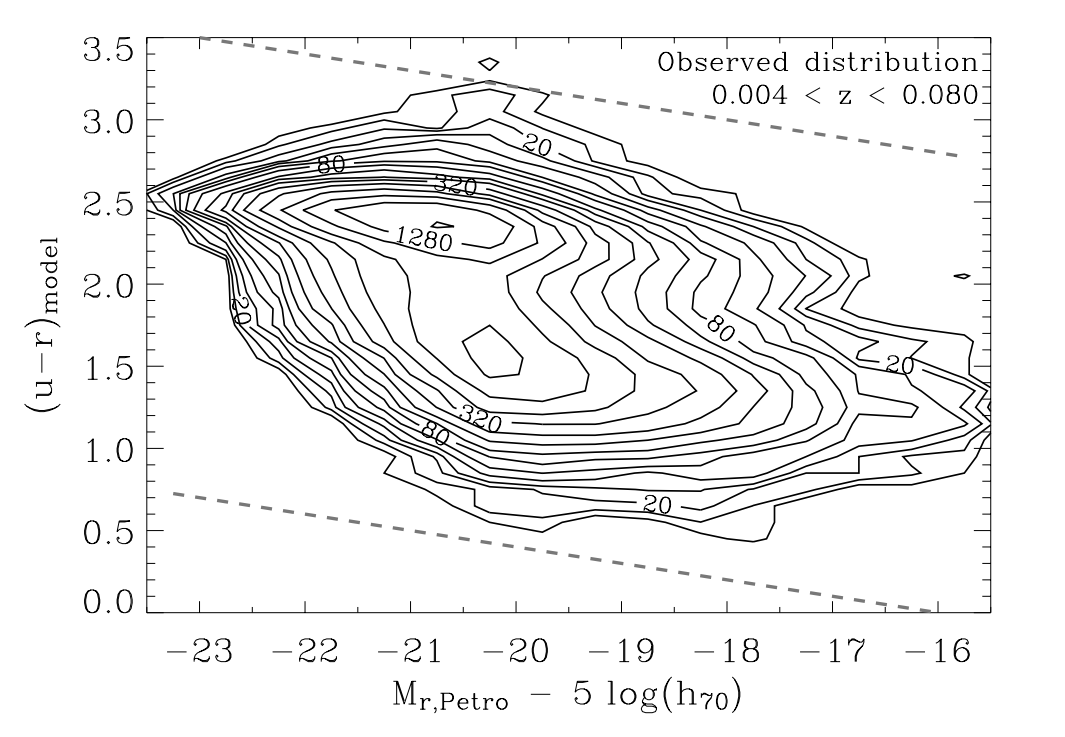
\includegraphics[width=0.475\textwidth]{baldry.png}}
\caption{Bimodality in the colour-magnitude diagram from \citet{Baldry04} (Figure 1) for 66,846 galaxies total. The contours are determined for galaxy number counts in 0.1 colour x 0.5 magnitude bins and are on a logarithmic scale, starting at 10 and doubling every two contours. Note that the $x$-axis is not flipped, therefore the most massive objects are found on the left of the plot.}
\label{baldry}
\end{figure}


The sparsely populated colour space between these two populations, the so-called `green valley', provides clues to the nature and duration of galaxies' transitions from blue to red. These transitions must occur on rapid timescales, otherwise an accumulation of galaxies residing in the green valley would be found, rather than an accumulation in the red sequence as is observed \citep{Arnouts07, Martin07}. Green valley galaxies have therefore long been thought of as the `crossroads' of galaxy evolution; a transition population between the two main galactic stages of the star forming blue cloud and the `dead' red sequence \citep{Bell04, Wyder07, Schim07, Martin07, Faber07, Mendez11, Gonc12, Sch2014}. 

The intermediate colours of these green valley galaxies have been interpreted as evidence for recent quenching (suppression) of star formation \citep{Salim07}. Star forming galaxies are observed to lie on a well defined mass-SFR relation, however quenching a galaxy causes it to depart from this relation (\citealt{Noeske07, Peng}; see Figure \ref{sfr_mass_sub})

By studying the galaxies which  have just left this mass-SFR relation, the quenching mechanisms by which this occurs can be probed. There have been many previous theories for the initial triggers of these quenching mechanisms, including negative feedback from AGN \citep{Sch07}, mergers \citep{Darg10a}, supernovae winds \citep{MFB12} and secular evolution \citep{Masters10, Masters11}. In particular observations of AGN host galaxies reveal their location in the green valley, suggesting a particular role for AGN feedback in the process of quenching \citep{Nandra07, Hasinger08, Silverman08, Sch2014}. Direct observations have also been made of the decline of the sSFR of a galaxy with black hole accretion \citep{Sch07, Wild07, Nandra07}, which is theorised to occur due to the shock heating of gas from active black hole ejecta. By investigating the \emph{amount} of quenching that has occurred between the blue cloud, green valley and red sequence, constraints to these quenching mechanism theories can be applied. 
\begin{table*}
\begin{tabular*}{0.9\textwidth}{r| @{\extracolsep{\fill}}cccc}
\hline
\begin{tabular}[c]{@{}c@{}} {\color{white} -} \\ {\color{white} -}  \end{tabular} & All                                                      & Red Sequence                                              & Green Valley                                              & Blue Cloud \\  \hline 
Smooth-like ($p_s > 0.5$)        & \begin{tabular}[c]{@{}c@{}}42453\\ (33.6\%)\end{tabular} & \begin{tabular}[c]{@{}c@{}}17424\\ (13.8\%)\end{tabular}  & \begin{tabular}[c]{@{}c@{}}10687\\ (8.4\%)\end{tabular}   & \begin{tabular}[c]{@{}c@{}}14342\\ (11.3\%)\end{tabular}  \\ 
Disc-like ($p_d > 0.5$)          & \begin{tabular}[c]{@{}c@{}}83863\\ (66.4\%)\end{tabular} & \begin{tabular}[c]{@{}c@{}}10722\\ (8.4\%)\end{tabular}   & \begin{tabular}[c]{@{}c@{}}13257\\ (10.5\%)\end{tabular}  & \begin{tabular}[c]{@{}c@{}}59884\\ (47.4\%)\end{tabular}  \\
Early-type ($p_s \geq 0.8$) & \begin{tabular}[c]{@{}c@{}}10517\\ (8.3\%)\end{tabular}  & \begin{tabular}[c]{@{}c@{}}5337\\ (4.2\%)\end{tabular}    & \begin{tabular}[c]{@{}c@{}}2496\\ (2.0\%)\end{tabular}    & \begin{tabular}[c]{@{}c@{}}2684\\ (2.1\%)\end{tabular}    \\
Late-type ($p_s \geq 0.8$)  & \begin{tabular}[c]{@{}c@{}}51470\\ (40.9\%)\end{tabular} & \begin{tabular}[c]{@{}c@{}}4493\\ (3.6\%)\end{tabular}    & \begin{tabular}[c]{@{}c@{}}6817\\ (5.4\%)\end{tabular}    & \begin{tabular}[c]{@{}c@{}}40430\\ (32.0\%)\end{tabular}  \\ \hline
\textbf{Total}                       & \begin{tabular}[c]{@{}c@{}}\textbf{126316} \\ (100.0\%)\end{tabular}                                                & \begin{tabular}[c]{@{}c@{}}28146 \\ (22.3\%)\end{tabular} & \begin{tabular}[c]{@{}c@{}}23944 \\ (18.9\%)\end{tabular} & \begin{tabular}[c]{@{}c@{}}74226 \\ (58.7\%)\end{tabular} \\\hline
\end{tabular*}
\caption{Table showing the break down of the GZ2 sample into the subsets of the colour-magnitude diagram by galaxy type.}
\label{subs}
\end{table*}

I have been motivated by a recent result suggesting two contrasting evolutionary pathways through the green valley by different morphological types \cite[hereafter S14]{Sch2014} specifically that late-type galaxies quench very slowly and form a nearly static disc population in the green valley, whereas early-type galaxies quench very rapidly, transitioning through the green valley and onto the red sequence in $\sim 1$~Gyr. That study used a toy model to examine quenching across the green valley; I implement a simple novel method utilising Bayesian statistics (for a comprehensive overview of Bayesian statistics see either \citealt{MacKay} or \citealt{Sivia}) in order to find the typical model parameters of the star formation history of galaxies in a given population. Previous investigations have only implemented frequentist methods on small sample sizes; however here I implement Bayesian methods on large populations of galaxies to determine the evolution. I assume the simplest model possible in order to derive any useful information before implementing more sophisticated techniques in future work. 

%We have been motivated by a previous Galaxy Zoo investigation by  \cite[hereafter S14]{Sch2014}, who by using a toy model found two contrastingly different evolutionary pathways between morphological types across the green valley. Their conclusions suggested that late-type (disc-like) galaxies quench very slowly due to gas depletion across the blue cloud until they reach the green valley after several gigayears with little morphological changes (suggesting a static disc population in the green valley); whereas early-type (smooth-like) galaxies quench very rapidly, triggering a morphological change and transitioning to the red sequence in $\sim 1~\rm{Gyr}$. Unlike this previous study, this investigation implements a novel method utilising Bayesian statistics (for a comprehensive overview of Bayesian statistics see either \citealt{MacKay} or \citealt{Sivia}) in order to find the most likely model description of the star formation histories of galaxies in the three populations. It also provides a direct comparison with our current understanding of galaxy evolution from stellar population synthesis (SPS, see section \ref{SPS}) models. 



%Through this approach, we aim to determine the following:
%\begin{enumerate}
%\item What previous star formation history (SFH) causes a galaxy to reside in the green valley at the current epoch?
%\item Why is the green valley so sparsely populated?
%\item Is the green valley a transitional or static population? 
%\item If the green valley is a transitional population then how many routes through it are there? 
%\item Are there morphological dependent differences between these routes through the green valley? 
%\end{enumerate}

This report proceeds as follows. Section \ref{data} contains a description of the sample data, models and simple Bayesian methods used in this initial analysis. Section \ref{results} highlights the early and most recent results, with Section \ref{thesis} providing a detailed discussion of how this work will develop throughout the next two years. These preliminary findings are summarised in Section \ref{conc}. The zero points of all ugriz magnitudes are in the AB system and where necessary I adopt the WMAP Seven-Year Cosmological parameters \citep{WMAP} with $(\Omega_m, \Omega_{\lambda}, h) = (0.26, 0.73, 0.71)$. 

\section{Data and Models}\label{data}

\subsection{Morphological Classification \& Galaxy Zoo}
%Previously, Hubble & DeV
%Small sample sizes 
%Binary classifications - smooth or disc, yes or no - decisions to be made 
% Statistically poor due to low numbers of classifiers 
Visual classification of galaxies by shape was pioneered by \citet{Hubble26} by his famous `tuning fork' system and has since progressed through more elaborately proposed systems of classification of \citet{deV59} and \citet{Sandage75}. A common feature of all systems however is the separation of galaxies into the two broad classes of \emph{disc} and \emph{elliptical} galaxies. Due to the massive variety in the shapes, structures and viewing angles of galaxies, classification has always been a distinctly manual task (although attempts to automate it have been made, with much less success, see \citealt{NA10}) for which great effort must be instilled in order to accrue large sample sizes. This has been done for a range of sample sizes by a small number of observers; from clusters \citep{Dressler80, SB84, Smail97, Michard08}, to $14,000$ galaxies \citep{NA10} up to $48,000$ galaxies \citep{Sch07}. These samples have been used to study the morphological dependency of galaxy evolution with varying degrees of agreement, however are incomplete for the following reasons:
\begin{enumerate}
\item limited sample sizes leading to insufficient statistics,
\item unreliable classifications from single or small number of users,
\item the binomial nature of the concurrent classifications. 
\end{enumerate}

Statistically significant studies of the morphological dependancy of galaxy evolution were therefore not possible with these samples. Galaxy Zoo \citep{Lintott08} is a web interface which originally asked non-scientists to help classify 1 million SDSS DR7 galaxy images. The advent of Galaxy Zoo led to a morphologically classified galaxy sample which was large in size and had at least 40 separate users classify each image. This led to a probabilistic classification system which was continuous rather than discrete.

In this investigation I utilise visual classifications of galaxy morphologies from the Galaxy Zoo 2\footnote{\url{http://zoo2.galaxyzoo.org/}} citizen science project \citep{GZ2}; for which the full question tree for each image is shown in Figure 1 of \citet{GZ2}.  Specifically, the Galaxy Zoo 2 \citep{GZ2} project consists of $304, 022$ images from the SDSS DR8 (a subset of those classified in Galaxy Zoo 1; GZ1) all classified by \emph{at least} 17 independent users, with the mean number of classifications standing at $\sim42$. The GZ2 project provides much more detailed classifications than the GZ1 project, allowing for further investigation of specific galaxy classes in the future with this investigation (see Section \ref{thesis}). 
%The GZ2 sample is more robust than the GZ1 sample and provides more detailed morphological classifications, including features such as bars, the number of spiral arms and the ellipticity of smooth galaxies. 

%The only further selection that was made to the sample was for the removal of  objects considered to be stars or artefacts by the users (i.e. with $p_{star/artefact} ~\geq~ 0.8$). Further to this, we required NUV photometry from the GALEX survey, within which $\sim42\%$ of the GZ2 sample were observed, giving a total sample size of $126, 316$ galaxies. 

%The first task asks users to chose whether a galaxy is mostly smooth, is featured or is a star/artefact. Unlike other tasks further down in the decision tree, every user who classifies a galaxy image will complete this task (others, such as whether the galaxy has a bar, is dependent on a user having first classified it as a featured galaxy), therefore we have very statistically robust classifications at this level.

The classifications from users produces a vote fraction for each galaxy (the debiased fractions calculated by \citet{GZ2} were used in this investigation); for example if 80 of 100 people thought a galaxy was disc shaped, whereas 20 out of 100 people thought the same galaxy was smooth in shape (i.e. elliptical), that galaxy would have vote fractions $p_{s} = 0.2$ and $p_{d} = 0.8$. In this example this galaxy would be included in the \emph{`clean'} disc sample ($p_d \geq 0.8$) according to \cite{GZ2} and would be considered a late-type galaxy. These vote fractions allow each galaxy to be considered in a large statistical analysis of how smooth and disc galaxies differ in their SFHs; the like of which has not been possible prior to this investigation.

\begin{figure}
\centering{
\includegraphics[width=0.45\textwidth]{col_mag_with_GV.pdf}}
\caption{Colour-magnitude diagram for the Galaxy Zoo 2 population showing the definition between the blue cloud and the red sequence from \citet{Baldry04} with the dashed line. The solid lines show $\pm 1\sigma$ either side of this definition; any galaxy within the boundary of these two solid lines is considered a green valley galaxy.}
\label{CMGV}
\end{figure}

To define which of my sample of $126, 316$ galaxies were in the green valley, I looked to previous definitions in the literature defining the separation between the red sequence and blue cloud. \citet{Baldry04} used local galaxies from the SDSS to trace this bimodality by fitting double Gaussians to the colour magnitude diagram without cuts in morphology. Their relation is definite in their equation 11 as:
\begin{equation}
C'_{ur}(M_{r}) = 2.06 - 0.244 \tanh \left( \frac{M_r + 20.07}{1.09}\right)
\end{equation}
and is shown in Figure \ref{CMGV} by the dashed line. Any galaxy within $\pm 1\sigma$ of this line, shown by the solid lines in Figure \ref{CMGV}, is therefore considered a green valley galaxy. The decomposition of the sample into red sequence, green valley and blue cloud galaxies is shown in Table \ref{subs} along with further subsections by galaxy type. This table also defines the definitions I adopt henceforth for early-type ($p_s~ \geq~0.8$), late-type ($p_d~ \geq~0.8$), smooth-like ($p_s~ >~0.5$) and disc-like ($p_d~ >~0.5$) galaxies. 


\subsection{Quenching Models}\label{quench}
The quenched star formation history (SFH) of a galaxy can be simply modelled as an exponentially declining star formation rate (SFR) across cosmic time ($0 \leq t ~\rm{[Gyr]} \leq 13.8$) as:
\begin{equation}\label{sfh}
SFR =
\begin{cases}
i_{sfr}(t_q) & \text{if } t < t_q \\
i_{sfr}(t_q) \times exp{\left( \frac{-(t-t_{q})}{\tau}\right)} & \text{if } t > t_q 
\end{cases}
\end{equation}
where $t_{q}$ is the onset time of quenching, $\tau$ is the timescale over which the quenching occurs and $i_{sfr}$ is an initial constant star formation rate dependent on $t_q$.  A smaller $\tau$ value corresponds to a rapid quench, whereas a larger $\tau$ value corresponds to a slower quench. 

I make the assumption that all galaxies formed at a time $t=0~\rm{Gyr}$ with an initial burst of star formation. The mass of this initial burst is controlled by the value of the $i_{sfr}$ which is set as the average sSFR at the time of quenching $t_q$. \citet{Peng} defined a relation (their equation 1) by empirically fitting to SDSS data for the average sSFR and redshift (cosmic time, t) as:
\begin{equation}
sSFR(m,t) = 2.5 \left( \frac{m}{10^{10} M_{\odot}} \right)^{-0.1} \left(\frac{t}{3.5}\right)^{-2.2} \rm{Gyr}^{-1}.
\end{equation}
Beyond $z \sim 2$ the characteristic SFR flattens and is roughly constant back to $z\sim6$. The cause for this change is not well understood but can be seen across similar observational data \citep{Peng, Gonzalez, Beth}. Motivated by these observations, I take the relation as defined in \citet{Peng} up to a cosmic time of $t=3~\rm{Gyr} (z \sim 2.3)$ and prior to this assume a constant average SFR (see Figure \ref{sfr_mass_col}). At the point of quenching, $t_{q}$, the models are defined to have a SFR which lies on this relationship for the sSFR, for a galaxy with mass, $m = 10^{10.27} M_{\odot}$ (the mean mass of the GZ2 sample; see Figure \ref{sfr_mass_col}.
 
%Under these assumptions the average SFR of our models will result in a lower value than the relation defined in \citet{Peng} at all cosmic times with this treatment; each galaxy only resides on the `main sequence' at the point of quenching. However galaxies cannot remain on the `main sequence' from early to late times throughout their entire lifetimes given the unphysical stellar masses and SFRs this would result in at the current epoch in the local Universe \citep{Beth, Heinis14}. If we were to include prescriptions for no quenching, starbursts, mergers, AGN etc. into our models we would improve on our reproduction of the average SFR across cosmic time; however in the interest of Occam's razor \citep{Sivia, Sok02} we have focussed on the simplest model possible.

Once this evolutionary SFR is obtained, I convolve it with the \citet{BC03} population synthesis models to generate a model SED at each time step. Fluxes from stars younger than $3~$Myr are suppressed to mimic the large optical depth of protostars embedded in dusty formation cloud. Filter transmission curves are then applied to obtain AB magnitudes and therefore predicted colours. The right panel of Figure \ref{sfr_mass_col} shows the evolution of these colours from the point of quenching onwards in the optical-NUV colour space.

Given that information about these modelled populations is available across all cosmic time, they can be `observed' at a given time in their history; this correlates with the observed redshfit of the GZ2 sample given the modelling assumptions.
%therefore, if the models were real populations, this would correlate with a measurable redshift. This `observed' time $t^{obs}$ can be thought of as a galaxy's age, as we make the assumption that all galaxies form with an initial burst of star formation at $t=0$. Therefore, for the GZ2 sample, the observed redshift was used to calculate the assumed age of each galaxy, in order to compare the observed colours to the predicted models colours directly. 

\subsection{Bayesian Techniques}
In order to achieve robust conclusions I conduct a a fully Bayesian analysis \citep{Sivia, MacKay} of the SFH models in comparison to the observed GZ2 sample data. This approach requires consideration of all possible combinations of $\theta \equiv (t_{q}, \tau)$. %which will be distributed with a mean, $\mu$ and standard deviation, $\sigma$, so that:
%\begin{equation}
%w = (\mu_{\theta}, \sigma_{\theta}) = (\mu_{t_{q}}, \sigma_{t_{q}}, \mu_{\tau}, \sigma_{\tau})
%\end{equation}
%Defining the Bayesian probability for a combination of $\theta$ values \underline{given} what we know about $w$: $P(\theta|w) = P(t_{q}, \tau|w) = P(t_{q}|w)P(\tau|w)$, gives:
%\begin{multline}\label{prior}
%P(\theta|w) = \frac{1}{\sqrt[]{4\pi^2\sigma^2_{t_{q}}\sigma^2_{\tau}}} \exp\left[-\frac{(t_{q}-\mu_{t_{q}})^2}{2\sigma^2_{t_{q}}}\right] \\ \exp\left[-\frac{(\tau-\mu_{\tau})^2}{2\sigma^2_{\tau}}\right].
%\end{multline}
%Here we assume that $ P(t_{q}|w)$ and $P(\tau|w)$ are independent of each other, as we have no prior knowledge of how these two parameters are related. Perhaps if we were to investigate a specific mechanism, for which we knew the quenching timescale and the epoch at which it is most common then we may assume otherwise. However, since we are attempting to investigate quenching mechanisms as a whole we make the simplest assumption for our prior and take a broad Gaussian distribution across both parameter spaces. 

\begin{figure*}
\centering{
\includegraphics[width=0.9\textwidth]{sfr_mass_subsets.pdf}}
\caption{A novel plot showing the star formation rate versus stellar mass diagrams for the different populations of galaxies  (top row, left to right: all galaxies, GZ2 `clean' disc and smooth galaxies; bottom row, left to right: blue cloud, green valley and red sequence galaxies). Their contributions to the star forming `sequence' (from \citet{Peng}, shown by the solid blue line with 0.3 dex scatter by the dashed lines) are shown. The green valley does appear to be a transitional population between the blue cloud and the red sequence. Detailed analysis of star formation histories can elucidate the nature of the different populations' pathways through the green valley.}
\label{sfr_mass_sub}
\end{figure*}

The likelihood of all of the GZ2 data ($\underline{d}$) \underline{given} a SFH model, i.e. a single combination of $\theta$ values, $P(\underline{d}|\theta, t_{k}^{obs})$ is then:
\begin{equation}
P(\underline{d}|\theta, t_{k}^{obs}) = \prod_{k} P(d_{k}|\theta, t_{k}^{obs}),
\end{equation}
where $d_{k}$ is a single data point of one galaxy. Assuming that all galaxies formed at $t=0~\rm{Gyr}$ with an initial burst of star formation, the `age' of each galaxy in the GZ2 sample is equivalent to an observed time, $t^{obs}_{k}$ or observed redshift. I then use this `age' to calculate the predicted model colours at this cosmic time for a given combination of $\theta$: $d_{c,p}(\theta, t^{obs}_{k})$ for both optical $(c=opt)$ and NUV $(c=NUV)$ colours. The model colours can now be directly compared with the observed GZ2 galaxy colours, so that for a single galaxy k with optical ($u-r$) colour, $d_{opt, k}$ and NUV ($NUV-u$) colour, $d_{NUV,k}$, the Bayesian probability $P(d_{k}|\theta, t^{obs}_{k})$ is:


\begin{multline}\label{like}
P(d_{k}|\theta, t^{obs}_{k}) = \frac{1}{\sqrt{2\pi\sigma_{opt, k}^2}}\frac{1}{\sqrt{2\pi\sigma_{NUV, k}^2}} \\ \exp{\left[ - \frac{(d_{opt, k} - d_{opt, p}(\theta, t_{k}^{obs}))^2}{\sigma_{opt, k}^2} \right]} \\ \exp{\left[ - \frac{(d_{NUV, k} - d_{NUV, p}(\theta, t_{k}^{obs}))^2}{\sigma_{NUV, k}^2} \right]},
\end{multline}

The assumptions here are that: $P(d_{opt}|\theta, t^{obs}_{k})$ and $P(d_{NUV}|\theta, t^{obs}_{k})$ are independent of each other and that galaxies of a given population are the same, therefore can be described by a single quenching model, $\theta$. I also do not consider the effects of intrinsic scatter in the data.
%as with $t$ and $\tau$ in Equation \ref{prior}. As previously we do not believe we can set a sensible prior to these parameters unless we were to investigate a specific quenching mechanism.
%
%Equation \ref{like} gives us the probability of the data \underline{given} a specific model. However what we need is the probability of each combination of $\theta$ values \underline{given} the GZ2 data: $P(\theta|\underline{d}, t^{obs}, w)$, i.e. how likely is a single SFH model given the observed colours of all of the GZ2 galaxies. We can find this by:
The posterior function can then be calculated from this likelihood, where $P(\theta)$ is the prior on $\theta$, which is assumed to be flat across the parameter space:
\begin{equation}\label{big}
P(\theta|\underline{d}, t,^{obs}) = \frac{P(\underline{d}|\theta, \underline{t}^{obs})P(\theta)}{\int P(\underline{d}|\theta, \underline{t}^{obs})P(\theta) d\theta}.
\end{equation}


As the denominator of Equation \ref{big} is a normalisation factor, comparison between posterior values for two different  $\theta$ values is equivalent to a comparison of the numerators. Calculation of $P(\theta|\underline{d}, \underline{t},^{obs} w)$  for any $\theta$ is possible given data for the GZ2 sample (or a sub-sample thereof). Markov Chain Monte Carlo (MCMC; \citealt{MacKay, Dan, GW10}) provides a robust comparison of the posterior function across relevant $\theta$ values without the need to explore the entire parameter space; here I choose a Python implementation of an affine invariant ensemble sampler by \cite{Dan}; \emph{emcee}.

%This method allows for a speedier exploration of the parameter space by avoiding those areas with low likelihood. A large number of `walkers' are started at an initial position where the likelihood is calculated, from there they individually `jump' to a new area of parameter space. If the likelihood in this new area is greater than the original position then the `walkers' retain this position. This new position then influences the direction of the  `jumps' of other walkers.  This is repeated for the defined number of steps until the `walkers' have found the regions of highest likelihood.
%
%It is expected that those subsets of galaxies with large numbers will rapidly converge the \emph{`walkers'} (see Section \ref{stats}) into the regions of high likelihood without the need to explore the whole parameter space. Conversely the smaller galaxy subsets will allow a full exploration of the parameter space. It is also expected that those subsets of galaxies with narrow ranges of either NUV or optical colours will also cause the \emph{`walkers'} to converge rapidly into the regions of high likelihood without the need to explore the whole of the parameter space. This raises the issue of whether the sampling method is capable of finding multiple likelihood peaks, however the Figures in Section \ref{results} show it is capable of finding multiple peaks in both parameters. 
%\begin{figure*}
%\includegraphics[width=0.4975\textwidth]{gv_smooth_clean.pdf}
%\includegraphics[width=0.4975\textwidth]{gv_disc_clean.pdf}
%\caption{Early (incorrect) result for galaxies in the Galaxy Zoo 2 sample defined as clean green valley galaxies, contour and histogram plots (all normalised over the same value) show the regions of greatest likelihood for an exponential model star formation history parameters $[t_{quench}$ and $\tau_{quench}]$ for both smooth-like(left) and disc-like (right) galaxies. $t_{q}$ is the time at which quenching occurs (Gyr) and $\tau_{q}$ is the time scale on which quenching occurs (Gyr; the larger the $\tau_{q}$, the slower the quenching). Background colours show the star formation rate predicted by this model after a time $t \sim 12.8~\rm{Gyr}$, which is the average observed time of the galaxies in the GZ2 sample. Galaxies contribute  to $[t_{q}, \tau_{q}]_{smooth}$ and $[t_{q}, \tau_{q}]_{disc}$ according to their Galaxy Zoo 2 vote fraction (i.e. a galaxy with $p_{disc} \sim p_{smooth} \sim 0.5$ will contribute equally to each set of parameters). These contours are the result of the `burn-in' step for MCMC methods.}
%\label{gv_clean}
%\end{figure*}

\begin{figure*}
\centering{
\includegraphics[width=\textwidth]{sfr_mass_colour_diagram.pdf}}
\caption{Left panel: SFR against stellar mass for all the sample galaxies (shaded contours), with model galaxy trajectories shown as coloured points/lines. The SFHs of the models are shown in the middle panel, where the SFR is initially constant before quenching at time $t$ and thereafter exponentially declining with a characteristic timescale $\tau$. I set the SFR at the point of quenching to be consistent with the typical SFR of a star-forming galaxy at the quenching time, $t$ (dashed line; \citealt{Peng}). The full range of models reproduces the observed colour-colour properties of the sample (right panel); for clarity the figures show only 4 of the possible models explored in this study.}
\label{sfr_mass_col}
\end{figure*}

In addition to the colours, the GZ2 data provides uniquely powerful measurements of a galaxy's morphology. Previous galaxy classifications have been purely binary; either a galaxy is classified as smooth or as a disc by a single classifier or a consensus of classifiers. The GZ2 classifications however are continuous rather than discrete and can provide a measure of how `smooth-like' or `disc-like' a galaxy  is through the vote fractions obtained from a large number of users. Therefore the user vote fractions are incorporated into the sampling by considering them as weights to the likelihood $P(d_{k}|\theta, t^{obs}_{k})$ to which a single galaxy contributes to the posterior function. 
 %If either of these fractions is over $80\%$ then the galaxy is considered to be in the `clean' smooth or disc sample according to \citet{GZ2}. 

%If we ran the above sampling method on galaxies in either of the \emph{clean} samples, we would lose all the information about the intermediate galaxies and how these contribute to the likelihood of $P(\theta|\underline{d})$. It is the intermediate galaxies which are thought to be crucial to the morphological changes between early- and late-type galaxies; if this change is associated with the green valley in any way then these vote fractions contain information we wish to keep in our analysis. It was the consideration of these intermediate galaxies which was excluded from the investigation in S14.

%Therefore the likelihood can now be thought of as:
%\begin{equation}
%P(\underline{d}|\theta, \underline{t}^{obs}) = \prod_{k} p_{k} P(d_{k}|\theta, t_{k}^{obs}),
%\end{equation}
%
%where $p_{k}$ is either $p_{s}$ or $p_{d}$ for a single galaxy, k. We can then run the code with the GZ2 sample along with firstly, the $p_{s}$ vote fractions to find the most likely parameters for $\theta$ for smooth-like galaxies and secondly, with the $p_{d}$ vote fractions to find the most likely parameters for $\theta$ for disc-like galaxies. However, we find it more convenient to 

I therefore perform sampling across four parameters: $\theta = (t_{s}, \tau_{s}, t_{d}, \tau_{d}) = (\theta_{s}, \theta_{d})$ so that the likelihood function becomes:
\begin{equation}
P(\underline{d}|\theta, \underline{t}^{obs}) = \prod_{k} \left [p_{s, k} P(d_{k}|\theta_{s}, t_{k}^{obs}) + p_{d, k} P(d_{k}|\theta_{d}, t_{k}^{obs}) \right].
\end{equation}

%The \emph{emcee} algorithm searches through the parameter space to find the region that maximises $P(\theta|\underline{d})$ to return four parameter values for $t_{s}, \tau_{s}, t_{d}$ and $\tau_{d}$. If we find that $\theta_{s} ~\sim~ \theta_{d}$ for the green valley galaxies then we can conclude that this area of the colour-magnitude diagram consists of a single population that all have a similar SFH. 


The \emph{emcee} algorithm searches through the parameter space to find the $\theta$ value that maximises the posterior function for a typical galaxy in a population. The model outlined above has been developed using the \emph{Python} programming language into a package named: \emph{StarfPy} which will be made freely available online\footnote{Work in progress code can be found at github.com/rjsmethurst/starfpy}. This code is currently being optimised in order to speed up the run time, with the possibility of using look-up tables generated from the SPS models to determine the predicted colours more easily during the Markov Chain. Using a look-up table drastically reduces the run-time from $\sim 10$ hours to $\sim 5$ minutes for a 500 step length burn-in and run. A complete understanding of the errors incurred with this approximation of a look up table will be necessary. 

Extensive testing of \emph{StarfPy} has been completed with colours generated from the quenched star formation history models, as defined in Equation \ref{sfh}, with known $\theta$ parameters. \emph{StarfPy} is capable of finding the correct parameter values regardless of morphological vote fractions, assumed errors on the colours, start position and location of $\theta$ in the parameter space. Larger errors allow for a fuller exploration of the degeneracies between the the optical and NUV colours, whereas smaller errors constrains the MCMC method to give tighter estimates of the $\theta$ parameters. 

\section{Results}\label{results}


As an initial investigation I produced Figure \ref{sfr_mass_sub} to show the SFR against the stellar mass for the observed GZ2 sample and the subsets of blue cloud, green valley and red sequence as well as for the `clean' disc and smooth galaxy samples (with GZ2 vote fractions of $p_d \geq 0.8$ and $p_s \geq 0.8$ respectively). This visualisation, split by morphological type and populations in the colour magnitude diagram, is the first of it's kind. The green valley galaxies are indeed a population which have either left, or begun to leave, the SFR-mass relation or have some residual star formation still occurring. Interestingly, comparing those galaxies which reside on the main sequence for each subset, the tail ends of these populations (the low and high mass  galaxies) are primarily made up of smooth galaxies as opposed to disc galaxies.

As a sanity check I produced the left panel in Figure \ref{sfr_mass_col} to show how well my quenched SFH models reproduce: (i) the observed relationship between the SFR and the mass of a galaxy for the GZ2 sample, including how at the time of quenching they reside on the SF vs. mass relationship shown by the solid black line for a galaxy of mass, $M = 10^{10.27} M_{\odot}$ and (ii) the observed colours of the GZ2 sample. 

%The contour plots in Figures \ref{all}-\ref{blue_c_clean} show the regions of high likelihood for the SFH model parameters $\theta = (t, \tau)$ for both smooth- and disc-like galaxies (left and right panels respectively) when considering the different subsets of the galaxies in the GZ2 sample. These plots were produced by \emph{Starfpy} using the output of the MCMC sampling method outlined in Section \ref{stats}. A `burn-in' of 100 steps was utilised initially and then run until the `walkers' had converged to one or more likelihoods peaks. The histograms show the distribution for the individual parameters and are normalised to the same value across all the Figures in this Section. The colours in the background are provided as a reference to the predicted SFR at the average look-back time of the GZ2 sample ($t^{obs}=12.8~\rm{Gyr}$, see Figure \ref{pred}). 
%
%We consider how these areas of highest likelihood for each parameter change when we consider different subsets of the GZ2 sample.

In the rest of this Section I will refer to rapid, intermediate and slow quenching timescales which correspond to ranges of $0.0 < \tau ~\rm{[Gyr]} < 1.0$, $1.0 < \tau ~\rm{[Gyr]} < 2.0$ and $2.0 < \tau ~\rm{[Gyr]} < 3.0$ respectively.
 
\begin{figure*}
\includegraphics[width=\textwidth]{peaks_non_clean.pdf}
\caption{The locations of the peaks in the parameter space found by \emph{StarfPy} for all red sequence, green valley and blue cloud smooth and disc galaxies; shown by the red, green and blue circle and diamond points respectively. The colours in the background show the SFR as predicted for each $\theta$ model by a time of $12.8$ Gyr, the average observed time of the GZ2 sample. Error bars are plotted, however the peaks are so well constrained that the errors are too small to be visible on this scale. The distribution of the posterior function for one of these peaks is shown in Figure \ref{peak_pop}.}
\label{peaks_non}
\end{figure*}

%\subsection{Early Results}
%Preliminary results were obtained for each of the subsets of the GZ2 sample using a burn-in of 100 steps and a run of 250 steps. Originally it was thought that the resulting contour plots, shown in Figure \ref{gv_clean} for clean green valley galaxies, showed the distribution of the posterior function in the parameter space. However a more complete knowledge of Bayesian and MCMC methods was then obtained at the Penn State Astrostatistics Summer School in June 2014. This apparent distribution was actually due to an insufficient `burn-in' length. Also the Bayesian model implemented would never be able to return a distribution; only the typical $\theta$ parameters for a given population (which could in fact be a double peaked if the population itself was bimodal) as one of the underlying assumptions is it that all galaxies within a population can be described by the same model. 

Multiple typical peaks for model $\theta$ parameters for red sequence, green valley and blue cloud populations were found with \emph{StarfPy} and are shown below in Figures \ref{peaks_non} and \ref{peak_pop}.  Considering the number of galaxies in each sample population, the peaks found are incredibly well constrained. The existence of multiple peaks across all the populations suggests that the intrinsic scatter in the data is important, therefore future extension of this model should include a quantification of this intrinsic scatter.  
%Table of values

The most obvious result from Figure \ref{peaks_non} is how the three populations trace each other across the parameter space; the red sequence quenches earlier than the green valley which quenches earlier than the blue cloud (if in fact the galaxies in the blue cloud have quenched) but at similar quenching timescales. This means that all populations are tracing the evolution to the red sequence, confirming that the green valley is indeed a transitional population between blue cloud and red sequence regardless of morphology. Currently as the green valley is observed, its main constituent, is very slowly evolving disc-like galaxies along with intermediate- and some smooth-like galaxies which manage to pass across it within $\sim 1.0-1.5~\rm{Gyr}$.

Those galaxies defined to be in the optical red sequence show a preference for intermediate quenching timescales at early times for the smooth-like galaxies and slow quenching timescales for the disc-like galaxies; confirming the results found by S14 for different quenching timescales for different morphologies. The peaks for the disc-like galaxies occupy areas that also have higher residual star formation occurring, suggesting that the disc galaxies which make up the red sequence seem to reside at its edge, on the border with the green valley. 

There is a lack of likelihood for rapid quenching timescales, $\tau < 1.0~\rm{Gyr}$, across all subsets of galaxies. This is most apparent in the disc parameters %(the right hand panels of Figures \ref{all} - \ref{blue_c_clean}) 
where peaks below this value are not detected for any population. For the smooth galaxies a peak is found in the smooth green valley galaxies for these extremely rapid quenching timescales, suggesting the mechanism which drives this quenching is not only less common than intermediate quenching, but that it only occurs for smooth-like galaxies (this is in agreement with the findings of S14, however they attribute this rapid quenching as the most common mechanism for smooth galaxies). This suggests that this rapid quenching mechanism causes a change in morphology from a disc- to a smooth-like galaxy as it traverses the colour-magnitude diagram through the green valley. It seems plausible therefore, that this rare, rapid quenching mechanism is due to major mergers.

\begin{figure}
\includegraphics[width=0.4975\textwidth]{peak_pop.pdf}
\caption{Distribution of the posterior function from \emph{StarfPy} in $\theta$ parameter space for one peak for the smooth green valley population, as shown by the middle circular, green point in the left hand plot of Figure \ref{peaks_non}. The solid blue lines denote the best fit location of the peak with estimated errors shown ether side by the dashed lines.}
\label{peak_pop}
\end{figure}

The green valley disc galaxies still show preference however for intermediate quenching timescales; no peak is detected at slow quenching timescales unlike for red sequence discs. Given enough time ($t\sim4-5\rm{Gyr}$), these disc galaxies will eventually fully pass through the green valley and make it out to the red sequence (the right panel of Figure \ref{sfr_mass_col} shows galaxies with $\tau > 1.0~\rm{Gyr}$ do not approach the red sequence within $3~\rm{Gyr}$ post quench). I therefore theorise that with enough cosmic time, eventually disc-like galaxies will come to populate the red sequence at comparable fractions to smooth-like galaxies. At the current epoch and at the timescales at which disc-like galaxies have peak $\theta$ values, a large number of red disc-like galaxies would not be expected. 

\citet{Bamford09} who, using GZ1 vote fractions of galaxies in the SDSS, found a significant fraction of high stellar mass red spiral galaxies in the field. This suggests that since these galaxies are mostly found in the field, where they will be isolated from the effects of interactions from other galaxies, the slow quenching mechanisms present in their preferred star formation histories must be due to secular processes; mechanisms internal to the galaxy, in the absence of sudden accretion or merger events \citep{KK04, Sheth12}.

Although intermediate quenching is the dominant mechanism across both morphological types, it cannot completely account for the quenching of disc galaxies. The preference for slow quenching timescales at early times is dominant for disc galaxies in the red sequence (and consequently traced by the green valley) results in galaxies with masses at the current epoch of $\log M_* \sim 11.3 M_{\odot} yr^{-1}$. S14 concluded that slow quenching timescales were the most dominant mechanism for disc galaxies, however I show that intermediate quenching timescales are equally dominant. 

I will aim to investigate the possibility that these intermediate quenching timescales are caused by gas rich major mergers, major mergers without black hole feedback and predominantly from minor mergers. This is supported by the findings of simulations of minor mergers, one of which by \citet{Lotz08} finds that the timescales for equal mass gas rich mergers with large initial separations range from $\sim 1.1-1.9~\rm{Gyr}$ and another of \citet{Lotz11}, who find that as the baryonic gas fraction in a merger with mass ratio's of 1:1-1:4 increases, so does the timescale of the merger from $\sim0.2~\rm{Gyr}$ (with little gas, as above for major mergers causing rapid quenching timescales) upto $\sim1.5~\rm{Gyr}$ (with large gas fractions). 

Such simulations, as in \citet{Lotz08} also show that the remnants of these equal mass gas rich disc mergers (wet disc mergers) are observable for $\ga1~\rm{Gyr}$ post merger and appear ``disc-like and dusty", which is consistent with an \emph{early-type spiral morphology} (or \emph{Sa}) classification.  Such galaxies are often observed to have spiral features with a dominant bulge, suggesting that such galaxies will divide the vote fractions of the GZ2 users producing $p_s \sim p_d \sim 0.5$. I believe this is why the intermediate quenching timescales are therefore the dominant features for both smooth and disc galaxies in all populations.

All of this evidence suggests that there are not just two routes for galaxies through the green valley but \emph{three}: with the smooth- ($1.0 < \tau < 1.5 ~\rm{Gyr}$), intermediate- ($1.5 < \tau < 2.0~\rm{Gyr}$) and disc-like ($\tau > 2.0~\rm{Gyr}$) galaxies each having different SFHs which lead them across the green valley, given enough cosmic time. Since S14 did not consider intermediate galaxies, their conclusions that there are 2 routes through the green valley for galaxies contradicts with my statements that their are three or more routes, dependent on whether a galaxy is early-, intermediate- or late-type. 



\section{Thesis Development}\label{thesis}


Since the majority of the development of \emph{StarfPy} is now complete I can begin to contemplate the flexibility of this model and it's future applications within this thesis work. This analysis could be utilised for galaxies observed at higher redshifts, for example with those galaxies classified in the GZ: Hubble Project (with Hubble Space Telescope photometry). This will require a detailed understanding of how visual classifications are affected with increasing distance or redshift. Structural details are lost by PSF smoothing and disc and elliptical galaxies become indistinguishable. One of the next steps for Galaxy Zoo is to ask users to classify galaxy simulation images which can be artificially redshifted in order to study how the probabilistic classification changes. I have been involved with the convolution and processing of these simulation images so that they are indistinguishable from images obtained with SDSS. 

Considering the number of magnitude bands available across the SDSS, further analysis will also be possible with a larger set of optical and NUV colours, providing further constraints or the model could also be matched to a measured SFR and stellar mass of an observed galaxy. I aim to tackle some key elements of the overarching theory of galaxy evolution with \emph{StarfPy} by determining any differences in star formation histories for:
\begin{enumerate}
\item barred vs. non-barred disc galaxies
\item merging/interacting galaxies vs. isolated galaxies
\item fast vs. slow rotating elliptical galaxies
\item cluster vs. field galaxies,
\item bulgeless vs. bulge dominated galaxies
\end{enumerate}
using the more detailed GZ2 classifications, the halo occupancy measure from \citep{Yang07} and the projected neighbour density $\Sigma$, from \citet{Baldry06}. I also hope to study the distribution of the SFH parameters in each subset of the magnitude-colour diagram by running \emph{StarfPy} on each individual galaxy in the sample (once optimised) and using Hierarchical Bayesian modelling and Importance Sampling (also including an estimate of the intrinsic scatter) to determine the hyper-parameters for a given population. An example of the posterior function for the $\theta$ parameters for one galaxy is shown in Figure \ref{im_one}. This will allow for the distribution of the posterior function across the parameter space to be determined. The development of the \emph{StarfPy} code into one that is fully publishable and reference-able is also a goal for the future. 

\begin{figure}
\includegraphics[width=0.5\textwidth]{im_one.pdf}
\caption{Contours and histograms showing the distribution of the posterior function across the $\theta$ parameter space for just one galaxy; DR7 Object ID: 587736940373737567, with $z=0.046$, $p_{d} = 0.99$ and $p_{s} = 0.01$. The SDSS image of the galaxy is shown in the top right corner. The solid blue lines denote the best fit location of the peak with estimated errors shown ether side by the dashed lines. Compare this with Figure \ref{peak_pop} which shows the result from \emph{StarfPy} for all galaxies in the a population. Notice the difference in range of the axes; the population is highly constrained due to the sheer number of galaxies being used to fit a $\theta$ value, however in the single galaxy case the full degeneracy of the space is explored. Future applications of \emph{StarfPy} will therefore include calculating this distribution for each galaxy in the GZ2 sample before combining the results hierarchically to find the hyper $\theta$ parameters for a population of galaxies.}
\label{im_one}
\end{figure}

The results found from this first investigation compliment an observing run at the Isaac Newton Telescope, La Palma from May 2014A, to obtain spectra and a run at the Discovery Channel Telescope, Arizona, USA to obtain deep imaging of bulgeless disc galaxies (identified by the users of GZ2) which have growing black holes. These objects contradict accepted theories for merger driven black hole evolution, as mergers consequently form a bulge at the centre of a galaxy. I will complete the data reduction of both the spectra and the deep images. The spectra will allow the determination of black hole masses for each galaxy, for which previous estimates showed might be comparable to the mass of the black hole in the centre of the Milky Way \citep{Simmons13}. This sample of bulgeless galaxies will help to determine how important AGN feedback is to the quenching of star formation; future work will include running \emph{StarfPy} on this sample along with control samples (bulge dominated systems, bulgeless galaxies without a black hole) to see if their star formation histories differ. Another objective is to take the deep imaging data of these galaxies, calculate the colours in various apertures and compare the star formation histories found with \emph{StarfPy} across the disc of the galaxy to determine if the AGN has a declining effect on the amount of quenching with distance from the centre. 

These observations will help to answer the questions raised by this investigation into green valley galaxies; how dominant is secular evolution in our Universe and do AGN cause a significant amount of quenching in galaxies?

%In particular, with further use of the robust, detailed GZ2 classifications, we believe that our module will be able to distinguish if there is any statistical difference in the star formation histories of barred vs. non-barred galaxies. This will require a simple swap of $p_s$ and $p_d$ with $p_{bar}$ and $p_{no bar}$ from the available GZ2 vote fractions. We believe that this will aid in the discussion of whether bars act to quench star formation (by funnelling gas into the galaxy centre) or promote star formation (by causing an increase in gas density as it travels through the disc) both sides of which have been fiercely argued \citep{Masters11, Masters12, Sheth05, Ellison11}. 
%
%Further application of the \emph{StarfPy} code could be to investigate the parameters for currently merging/interacting pairs to those galaxies classified as merger remnants from their degree of disturbance. This will allow a direct comparison of the impact of a merger on the star formation rate of a galaxy by comparing the before and after scenario's. 
%
%It also thought that depending on the initial conditions of a galaxy merger this can either produce a slow or fast rotator elliptical galaxy. Since slow rotators are on average more massive objects that they may result from major mergers (dry) on the red sequence \citep{Em11} , whereas fast rotators are obtained in simulations from gas rich (wet) mergers and can form more disc-like objects \citep{Em07}. By using a sample of fast and slow rotators as input galaxies we may even be able to detect a difference in the star formation histories of wet and dry mergers and in turn how these two separate populations of elliptical galaxies arose. 
%
%One of the key elements of an overarching theory of galaxy evolution is to explain how field and cluster galaxies evolve in comparison to each other. The projected neighbour density, $\Sigma$, from \citet{Baldry06} can be used as to weight the likelihoods for cluster and field galaxies (instead of the vote fractions from GZ2 for $p_s$ and $p_d$) to determine if there is a measurable statistical difference in their star formation histories. 

%What can we do that no one else can?
%Future plans...


\section{Conclusion}\label{conc}
Thus far I have used morphological classifications from the Galaxy Zoo 2 project to determine the typical morphological dependent quenched star formation histories of galaxies in a given population through a Bayesian analysis of a simple exponentially declining star formation rate model. This has been achieved through the development of a new Python code, \emph{StarfPy}. Using this I determined the most likely parameters for the quenching time, $t_q$ and quenching timescale $\tau$ in this model for galaxies across the blue cloud, green valley and red sequence. I find that the green valley is indeed a transitional population for all morphological types, however this transition proceeds slowly for the majority of disc-like galaxies and may rarely occur very rapidly for smooth-like galaxies. Future work will include an extension of this \emph{StarfPy} code which will then be used to investigate a possible cause of the quenching in these galaxies through observations of bulgeless galaxies with growing black holes. 

\section*{Acknowledgements}
The author would like to thank D. Forman-Mackey and P. Marshal for extremely useful Bayesian statistics discussions and J. Binney for an interesting discussion on the nature of quenching and feedback in disc galaxies. 
RS acknowledges funding from the Science and Technology Facilities Council Grant Code ST/K502236/1.
This research has  made use of NASA's ADS service and Cornell's ArXiv. 


\begin{thebibliography}{}
%\bibitem[\protect\citeauthoryear{Aihara et al.}{2011}]{Aihara11} Aihara, H. et al., 2011, ApJSS, 193, 29
\bibitem[\protect\citeauthoryear{Arnouts et al.}{2007}]{Arnouts07} Arnouts, S. et al., 2007, A\&A, 476, 137
\bibitem[\protect\citeauthoryear{Baldry et al.}{2004}]{Baldry04} Baldry, I. K. et al., 2004, ApJ, 600, 681
\bibitem[\protect\citeauthoryear{Baldry et al.}{2006}]{Baldry06} Baldry, I. K. et al., 2006, MNRAS, 373, 469
\bibitem[\protect\citeauthoryear{Ball, Loveday \& Brunner}{2008}]{BLB08} Ball, N. M., Loveday, J. \& Brunner, R. J., 2008, MNRAS, 383, 907
\bibitem[\protect\citeauthoryear{Bamford et al.}{2009}]{Bamford09} Bamford, S. P. et al., 2009, MNRAS, 393, 1324
%\bibitem[\protect\citeauthoryear{Barnes \& Hernquist}{1996}]{BH96} Barnes, J. E. \& Hernquist, L., 1996, ApJ, 471, 115
%\bibitem[\protect\citeauthoryear{Barnes}{2002}]{Barnes02} Barnes, J. E., 2002, MNRAS, 333, 481
\bibitem[\protect\citeauthoryear{Bell et al.}{2004}]{Bell04} Bell, E. F. et al., 2004, ApJ, 608, 752
%\bibitem[\protect\citeauthoryear{Bell et al.}{2006}]{Bell06} Bell, E. F. et al., 2006, ApJ, 652, 270
%\bibitem[\protect\citeauthoryear{Bell et al.}{2007}]{Bell07} Bell, E. F. et al., 2007, ApJ, 663, 834
\bibitem[\protect\citeauthoryear{B\'ethermin et al.}{2012}]{Beth} B\'ethermin, M. et al., 2012, ApJ, 757, L23
%\bibitem[\protect\citeauthoryear{Blanton et al.}{2005}]{Blanton05} Blanton, M. R. et al., 2005, AJ, 129, 2562
%\bibitem[\protect\citeauthoryear{Blanton \& Roweis}{2007}]{BR07} Blanton, M. R. \& Roweis, S., 2007, AJ, 133, 734
\bibitem[\protect\citeauthoryear{Brammer et al.}{2009}]{Brammer09} Brammer, G. B. et al., 2009, ApJ, 706, 173
%\bibitem[\protect\citeauthoryear{Brinchmann et al.}{2004}]{Brinch04} Brinchmann, J. et al., 2004, MNRAS, 351, 1151
\bibitem[\protect\citeauthoryear{Bruzual \& Charlot}{2003}]{BC03} Bruzual, G. \& Charlot, S., 2003, MNRAS, 344, 1000
%\bibitem[\protect\citeauthoryear{Bundy et al.}{2007}]{Bundy07} Bundy, K. et al., 2007, ApJL, 655, L5
%\bibitem[\protect\citeauthoryear{Bundy et al.}{2009}]{Bundy09} Bundy, K. et al., 2009, ApJ, 697, 1369
%\bibitem[\protect\citeauthoryear{Bundy et al.}{2010}]{Bundy10} Bundy, K. et al., 2010, ApJ, 719, 1969
\bibitem[\protect\citeauthoryear{Cardelli et al.}{1989}]{Cardelli89} Cardelli, J. A. et al., 1989, ApJ, 345, 245
%\bibitem[\protect\citeauthoryear{Casteels et al.}{2013}]{Casteels13} Casteels, K. et al., 2013, MNRAS, 429, 1051
%\bibitem[\protect\citeauthoryear{Chabrier et al.}{2003}]{Chab03} Chabrier, G., 2003, PASP, 115, 763
%\bibitem[\protect\citeauthoryear{Chen et al.}{2010}]{Chen10} Chen, X. Y. et al., 2010, A\&A, 515, 101
%\bibitem[\protect\citeauthoryear{Conroy, Gunn \& White}{2009}]{CGW09} Conroy, C., Gunn, J. E. \& White, M. 2009, ApJ, 699, 486
\bibitem[\protect\citeauthoryear{Darg et al.}{2010}]{Darg10a} Darg, D. et al., 2010a, MNRAS, 401, 1552
\bibitem[\protect\citeauthoryear{de Vaucouleurs}{1959}]{deV59} de Vaucouleurs, G., 1959, Handbuch der Physik, 53, 275
\bibitem[\protect\citeauthoryear{Dressler}{1980}]{Dressler80} Dressler, A., 1980, ApJSS, 42, 565
%\bibitem[\protect\citeauthoryear{Ellison et al.}{2011}]{Ellison11} Ellison, S. L. et al., 2001, MNRAS, 416, 2182
%\bibitem[\protect\citeauthoryear{Emsellem et al.}{2007}]{Em07} Emsellem, E. et al., 2007, IAU Symposium 235
%\bibitem[\protect\citeauthoryear{Emsellem et al.}{2011}]{Em11} Emsellem, E, et al., 2011, MNRAS, 414, 888
%\bibitem[\protect\citeauthoryear{Eminian et al.}{2008}]{Eminian08} Eminian, C. et al., 2008, MNRAS, 384, 930
\bibitem[\protect\citeauthoryear{Faber et al.}{2007}]{Faber07} Faber, S. M. et al., 2007, ApJ, 665, 265
%\bibitem[\protect\citeauthoryear{Falomo et al.}{2008}]{Falomo08} Falomo, R. et al., 2008, ApJ, 673, 694
%\bibitem[\protect\citeauthoryear{Falkenberg et al.}{2009}]{Falk09} Falkenberg, M. A. et al., 2009, MNRAS, 397, 1954
\bibitem[\protect\citeauthoryear{Foreman-Mackey et al.}{2013}]{Dan} Foreman-Mackey, D., Hogg, D. W., Lang, D., Goodman, J., 2013, PASP, 125, 306
%\bibitem[\protect\citeauthoryear{Genel et al.}{2008}]{Genel08} Genel, S. et al., 2008, ApJ, 688, 789
\bibitem[\protect\citeauthoryear{Goodman \& Weare}{2010}]{GW10} Goodman, J. \& Weare, J., 2010, CAMCS, 5, 65
\bibitem[\protect\citeauthoryear{Gon\c calves et al.}{2012}]{Gonc12} Gon\c calves, T. S. et al., 2012, ApJ, 759, 67
\bibitem[\protect\citeauthoryear{Gonz\'alez et al.}{2010}]{Gonzalez} Gonz\'alez, V. et al., 2010, ApJ, 713, 115
\bibitem[\protect\citeauthoryear{Hasinger}{2008}]{Hasinger08} Hasinger, G., 2008, A\&A, 490, 905
\bibitem[\protect\citeauthoryear{Hubble}{1926}]{Hubble26} Hubble, E. P., 1926, ApJ, 64, 321
%\bibitem[\protect\citeauthoryear{Heinis et al.}{2014}]{Heinis14} Heinis, S. et al., 2014, MNRAS, 437, 1268
%\bibitem[\protect\citeauthoryear{Hopkins}{2004}]{Hopkins04} Hopkins, A. M., 2004, ApJ, 615, 209
%\bibitem[\protect\citeauthoryear{Im et al.}{2002}]{Im02} Im, M. et al., 2002, ApJ, 571, 136
\bibitem[\protect\citeauthoryear{Jarosik et al.}{2011}]{WMAP} Jarosik, N. et al., 2011, ApJSS, 192, 18
%\bibitem[\protect\citeauthoryear{Kauffmann et al.}{2003}]{Kauff03} Kauffman, G. et al., 2003, MNRAS, 341, 33
%\bibitem[\protect\citeauthoryear{Kaviraj et al.}{2011}]{Kav11} Kaviraj, S. et al. 2011, MNRAS, 411, 2148
%\bibitem[\protect\citeauthoryear{Kaviraj}{2014}]{Kav14} Kaviraj, S., 2014, MNRAS, 440, 2944
\bibitem[\protect\citeauthoryear{Kormendy \& Kennicutt}{2004}]{KK04} Kormendy, J. \& Kennicutt, R. J., 2004, ARA\&A, 42, 603
%\bibitem[\protect\citeauthoryear{Kormendy et al.}{2010}]{Kormendy10} Kormendy, J. et al., 2010, ApJ, 723, 54
%\bibitem[\protect\citeauthoryear{Kriek et al.}{2010}]{Kriek10} Kriek, M. et al., 2010, ApJL, 722, L64
\bibitem[\protect\citeauthoryear{Lintott et al.}{2008}]{Lintott08} Lintott, C. J. et al., 2008, MNRAS, 389, 1179
\bibitem[\protect\citeauthoryear{Lintott et al.}{2011}]{Lintott11} Lintott, C. J. et al., 2011, MNRAS, 410, 166
\bibitem[\protect\citeauthoryear{Lotz et al.}{2008}]{Lotz08} Lotz, J. et al., 2008, MNRAS, 391, 1137
\bibitem[\protect\citeauthoryear{Lotz et al.}{2011}]{Lotz11} Lotz, J. et al., 2011, MNRAS, 742, 103
\bibitem[\protect\citeauthoryear{MacKay}{2003}]{MacKay} MacKay, D. J. C., 2003, \emph{Information Theory, Inference and Learning Algorithms}, Cambridge University Press, ISBN 978-0-521-64298-9
\bibitem[\protect\citeauthoryear{Marasco, Fraternali \& Binney}{2012}]{MFB12} Marasco, A., Fraternali, F. \& Binney, J. J., 2012, MNRAS, 419, 1107
\bibitem[\protect\citeauthoryear{Maraston}{2005}]{Maraston05} Maraston, C., 2005, MNRAS, 362, 799
%\bibitem[\protect\citeauthoryear{Marigo \& Girardi}{2007}]{MG07} Marigo, P. \& Girardi, L. 2007, A\&A, 469, 239
%\bibitem[\protect\citeauthoryear{Martin et al.}{2005}]{Martin05} Martin, D. C. et al., 2005, ApJ, 619, L1
\bibitem[\protect\citeauthoryear{Martin et al.}{2007}]{Martin07} Martin, D. C. et al., 2007, ApJS, 173, 342
\bibitem[\protect\citeauthoryear{Masters et al.}{2010a}]{Masters10} Masters, K. L. et al., 2010, MNRAS, 405, 783
\bibitem[\protect\citeauthoryear{Masters et al.}{2011}]{Masters11} Masters, K. L. et al., 2011, MNRAS, 411, 2026
%\bibitem[\protect\citeauthoryear{Masters et al.}{2012}]{Masters12} Masters, K. L. et al., 2012, MNRAS, 424, 2180
%\bibitem[\protect\citeauthoryear{Melbourne et al.}{2012}]{Mel12} Melbourne, J. et al., 2012, ApJ, 748, 47
\bibitem[\protect\citeauthoryear{Mendez et al.}{2011}]{Mendez11} Mendez, A. J. et al., 2011, ApJ, 736, 110
\bibitem[\protect\citeauthoryear{Michard \& Andreon}{2008}]{Michard08} Michard, R. \& Andreon S., 2008, A\&A, 490, 923
%\bibitem[\protect\citeauthoryear{Miller, Rose \& Cecil}{2011}]{MRC11} Miller, N. A., Rose, J. A. \& Cecil, G. 2011, ApJL, 727, L15
\bibitem[\protect\citeauthoryear{Nair \& Abraham}{2010}]{NA10} Nair, P. B. \& Abraham, R. G. 2010, ApJSS, 186, 427 
\bibitem[\protect\citeauthoryear{Nandra et al.}{2007}]{Nandra07} Nandra, K. et al., 2007, ApJ, 660, L11
\bibitem[\protect\citeauthoryear{Noeske et al.}{2007}]{Noeske07} Noeske, K. G. et al., 2007, ApJ, 660, L43
%\bibitem[\protect\citeauthoryear{Oh et al.}{2011}]{Oh11} Oh, K. et al., 2011, ApJS, 195, 13
%\bibitem[\protect\citeauthoryear{Padmanabhan et al.}{2008}]{Pad08} Padmanabhan, N. et al., 2008, ApJ, 674, 1217
\bibitem[\protect\citeauthoryear{Peng et al.}{2010}]{Peng} Peng, Y. et al., 2010, ApJ, 721, 193
%\bibitem[\protect\citeauthoryear{Robertson et al.}{2006}]{Rob06} Robertson, B. et al., 2006, ApJ, 645, 986
\bibitem[\protect\citeauthoryear{Robitaille et al.}{2013}]{Rob13} Robitaille, T. P. et al., 2013, A\&A, 558, A33
\bibitem[\protect\citeauthoryear{Salim et al.}{2007}]{Salim07} Salim, S. et al., 2007, ApJSS, 173, 267
\bibitem[\protect\citeauthoryear{Sandage}{1975}]{Sandage75} Sandage, A., 1975, \emph{Galaxies and the Universe: Stars and Stellar Systems}, University of Chicago Press, ISBN 0-22-645970-5
\bibitem[\protect\citeauthoryear{Sandage \& Binggeli}{1984}]{SB84} Sandage, A. \& Binggeli, B., 1984, AJ, 89, 919
\bibitem[\protect\citeauthoryear{Schawinski et al.}{2007}]{Sch07} Schawinski, et al., 2007, MNRAS, 382, 1415
\bibitem[\protect\citeauthoryear{Schawinski et al.}{2009}]{Sch09} Schawinski, K. et al., 2009, MNRAS, 396, 818
\bibitem[\protect\citeauthoryear{Schawinski et al.}{2014}]{Sch2014} Schawinski, K. et al., 2014 (arXiv: 1402.4814)
\bibitem[\protect\citeauthoryear{Schiminovich et al.}{2007}]{Schim07} Schiminovich, D. et al., 2007, ApJS, 173, 315
%\bibitem[\protect\citeauthoryear{Scoville et al.}{2007}]{Scoville07} Scoville, N. et al., 2007, ApJSS, 172, 1
%\bibitem[\protect\citeauthoryear{Sheth et al.}{2005}]{Sheth05} Sheth, K. et al., 2005, ApJ, 632, 217
\bibitem[\protect\citeauthoryear{Sheth et al.}{2012}]{Sheth12} Sheth, K. et al., 2012, ApJ, 758, 136
\bibitem[\protect\citeauthoryear{Silverman et al.}{2008}]{Silverman08} Silverman, J. D., et al. 2008, ApJ, 675, 1025
\bibitem[\protect\citeauthoryear{Simmons et al.}{2013}]{Simmons13} Simmons, B. D. et al., 2013, MNRAS, 429, 2199
\bibitem[\protect\citeauthoryear{Sivia}{1996}]{Sivia} Sivia, D. S., 1996, \emph{Data Analysis: A Bayesian Tutorial}, Oxford University Press, ISBN 0-19-851889-7
\bibitem[\protect\citeauthoryear{Skibba et al.}{2009}]{Skibba09} Skibba, R. A. et al., 2009, MNRAS, 399, 966
\bibitem[\protect\citeauthoryear{Smail et al.}{1997}]{Smail97} Smail, I. et al., 1997, ApJSS, 110, 213
\bibitem[\protect\citeauthoryear{Springel, Di~Matteo \& Hernquist}{2005}]{Springel05} Springel, V., Di Matteo, T. \& Hernquist, L., 2005, ApJ, 620, L79
%\bibitem[\protect\citeauthoryear{Soklakov}{2002}]{Sok02} Soklakov, A. N., 2002, (arXiv:math-ph/0009007)
\bibitem[\protect\citeauthoryear{Taylor}{2005}]{Taylor05} Taylor, M. B., 2005, ASP Conference Series, 347
%\bibitem[\protect\citeauthoryear{Tojeiro et al.}{2013}]{Toj13} Tojeiro, R. et al., 2013, MNRAS, 432, 359
\bibitem[\protect\citeauthoryear{Wild et al.}{2007}]{Wild07} Wild, V. et al., MNRAS, 381, 543
\bibitem[\protect\citeauthoryear{Willett et al.}{2013}]{GZ2} Willett, K. et al., 2014, MNRAS, 435, 2835
\bibitem[\protect\citeauthoryear{Willmer et al.}{2006}]{Willmer06} Willmer, C. N. A. et al., 2006, ApJ, 647, 853
\bibitem[\protect\citeauthoryear{Wyder et al.}{2007}]{Wyder07} Wyder, T. K. et al., 2007, ApJS, 173, 293
\bibitem[\protect\citeauthoryear{Yang et al.}{2007}]{Yang07} Yang, X. et al., 2007, ApJ, 671, 153
%\bibitem[\protect\citeauthoryear{York et al.}{2000}]{York00} York, D. G. et al., 2000, AJ, 120, 1579
\end{thebibliography}{}


\end{document}